\documentclass[prl,reprint,showpacs,floatfix,nofootinbib]{revtex4-1}
\usepackage{epsfig,graphics,float,amsmath,mathtools}
\usepackage[colorlinks=true,citecolor=blue]{hyperref}
\usepackage{microtype,setspace,siunitx,physics,epsfig,graphicx}
\usepackage[caption=false]{subfig}
\usepackage{xcolor}
\usepackage[export]{adjustbox}
\usepackage{nameref,physics}
\usepackage{blindtext}
\captionsetup[subfigure]{labelformat=brace}
\usepackage[english]{babel}
%\definecolor{originblue}{RGB}{139,255,167}
%\definecolor{origingreen}{HTML}{fdae61}


\begin{document}
\title{Generating Simulated Data for Machine Learning Training Sets: Particle and Topological Defect Identification and Tracking}

\date{\today}
\author{Adam~A.~S.~Green}
\author{Eric~N.~Minor}
\author{Stian~D.~Howard}
\author{Cheol Park}
\affiliation{Department of Physics and Soft Materials Research Center, University of Colorado, Boulder, Colorado, 80309, USA}


\begin{abstract}
    \blindtext{}
\end{abstract}

\maketitle

\section{Introduction}
%context (ag)
%\blindtext{}
% - Intro to Machine Learning
%   - What is it
%   - Why it's valuable to us
In experiments where data is collected through video capture, which then needs to be annotated, often one of the most prohibitive factors to analyzing data collected is found through the difficulty of analyzing images. In many cases, human analysis of hundreds or thousands of individual frames is required to create a significant plot to determine a result. This can be extraordinarily time intensive and inefficient to do on a large scale. We hope to remove the countless hours of repetitive human image annotation with a trained machine learning algorithm which will allow a researcher to focus on the physics of an experiment.

% - Intro to LC systems
%   - Basics of islands
Liquid crystal films are composed of discrete layers of aligned molecules. Molecules are effectively constrained to their individual layer while maintaining a fluid freedom within the layer. Regions where there is an inconsistency in the layer count are referred to as islands. Islands can be easily observed through a camera as regions of higher light intensity due to the higher reflectivity of the film in those regions. Islands will tend to move with the surrounding fluid allowing them to be used as a marker for the fluid movement

%   - Basics of topological-defects -- Adam needs to help with this.

% - Island tracking - current methods are inflexible/expensive(computation/human time)/difficult
% - Lack robust tool for multiple things (different scripts/methods for islands,defects, etc.)
% - We use 'off-the-shelf' code for ML
All of these methods are highly rigid, however. For every application (defect tracking, island tracking, different camera settings) significant modifications are needed to read the images, identify features, and new analysis pipelines outlined to process the information. We intend to make a general purpose pipeline that will work for all our experiments with minimal additional work. Additionally only off-the-shelf ML and tracking libraries are to be used, while all training data is to be simulated eliminating the need of human annotation to train the model. 

% - Applicability test with islands -- complex use/flexibility tested with defects
Island tracking, a relatively simple application of Machine Learning, allows for a simple test of the applicability of Machine Learning, trained on simulated data, on experimental data. Topological defect tracking, a high complexity problem, allows for testing the flexibility and robustness of the methodology.
%


\section{Experimental Systems}

To confirm the veracity of our trained neural networks, which are trained on simulation data, we need an accompanying experimental setup to validate the network with real experimental data of interest. 

\subsection{Island Data}
%Race track experiment
For testing island tracking, we use data for the racetrack experiment for which we have already characterized. 

To generate the islands and flow, a 'racetrack' shaped depression in a stainless steel block is used. A film is drawn using a slider over the depression leaving a film suspended over the depression. Flow is generated by injecting air into the side of the depression, and allowing it to escape through the bottom of the depression. The effect of this setup is a circulating airflow in the depression stimulating a similar flow in the film above. 

%This figure needs updating. Remove the image of the material zoomed in, replace with image of track and airflow and filming location.
\begin{figure}
  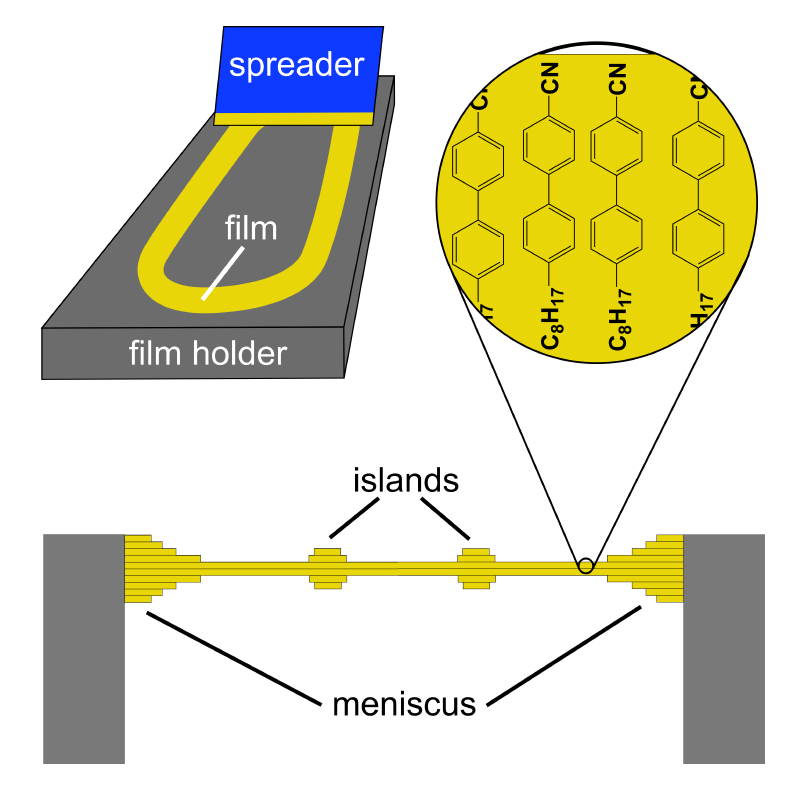
\includegraphics[width=\linewidth]{racetrack.png}
  \caption{Sketch of the racetrack setup}
  \label{fig:RaceTrackSketch}
\end{figure}

Islands are generated by aggressively stimulating the film with an extremely high flow rate. After islands are generated, the air injection rate is reduced to a spread of rates for the experiment. A Phantom V12.1 camera captures the reflected light from the film over a variety of frames per second (confirm actual value with racetrack paper). 

% Include a little more here. Another paragraph is needed. Perhaps about the expected flow pattern (pousille)?

\subsection{Defect Data}

At the center of our setup is a pressure chamber with an open aperture on the top to draw a film over. When pressure is provided to the chamber through a tube, the film balloons outward. A valve on the tube is then opened to the atmosphere, rapidly venting the pressure to the atmosphere. The valve is controlled by a computer program written to trigger the camera to start recording as well as track the pressure in chamber over time, all of which happens when a defined pressure difference between the chamber and atmosphere is achieved. 

% Confirm 

Smectic C liquid crystal films allow defects to be visualized with partially, or fully, crossed polarizers. In our setup, polarized light is shined perpendicularly onto the film. The reflected light is collected into a microscope where it passes through a partially crossed polarizer. Finally a high speed camera (Phantom V12.1) collects the images at 500 frames per second, and an exposure time of 1900 $\mu$s in gray-scale.

\begin{figure}
  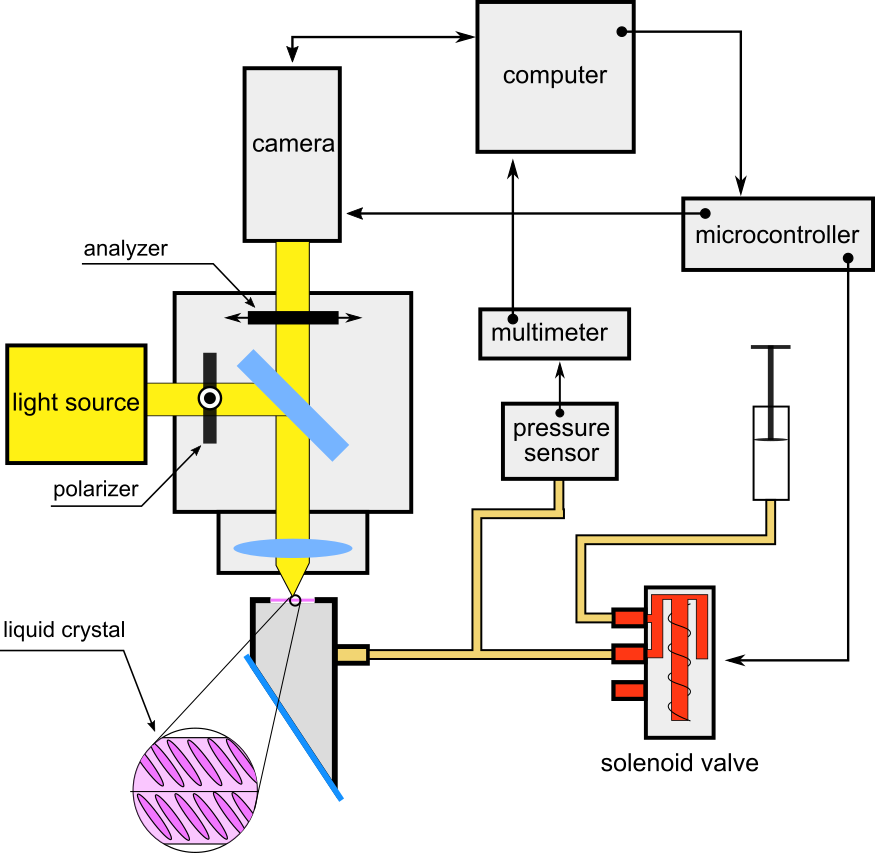
\includegraphics[width=\linewidth]{quench-schematic.png}
  \caption{Sketch of the quenching setup}
  \label{fig:Setup Sketch}
\end{figure}


Each video lasts a little over 12 seconds, capturing the entirety of the short term dynamics. Images are 1104x800  and have a 12 bit pixel grey scale precision, allowing for high contrast to be gained in post processing. When the polarizers are fully crossed, the reflected light is so dim that the images turn out fully black at the exposure time used -- a value which can't be increased due to the frame rate. Partially crossed polarizers allow for more light to reach the camera's CCD while still allowing for visualization of a defect.

For this experiment we're using a [material name - 'German material'] material to draw the film, which exists in a Smectic C phase at room temperatures. The heat chamber provides additional control of film state, allowing for faster annihilation of the defects at higher temperatures, or reduced island formation and noise at lower temperatures. 

\begin{figure}
  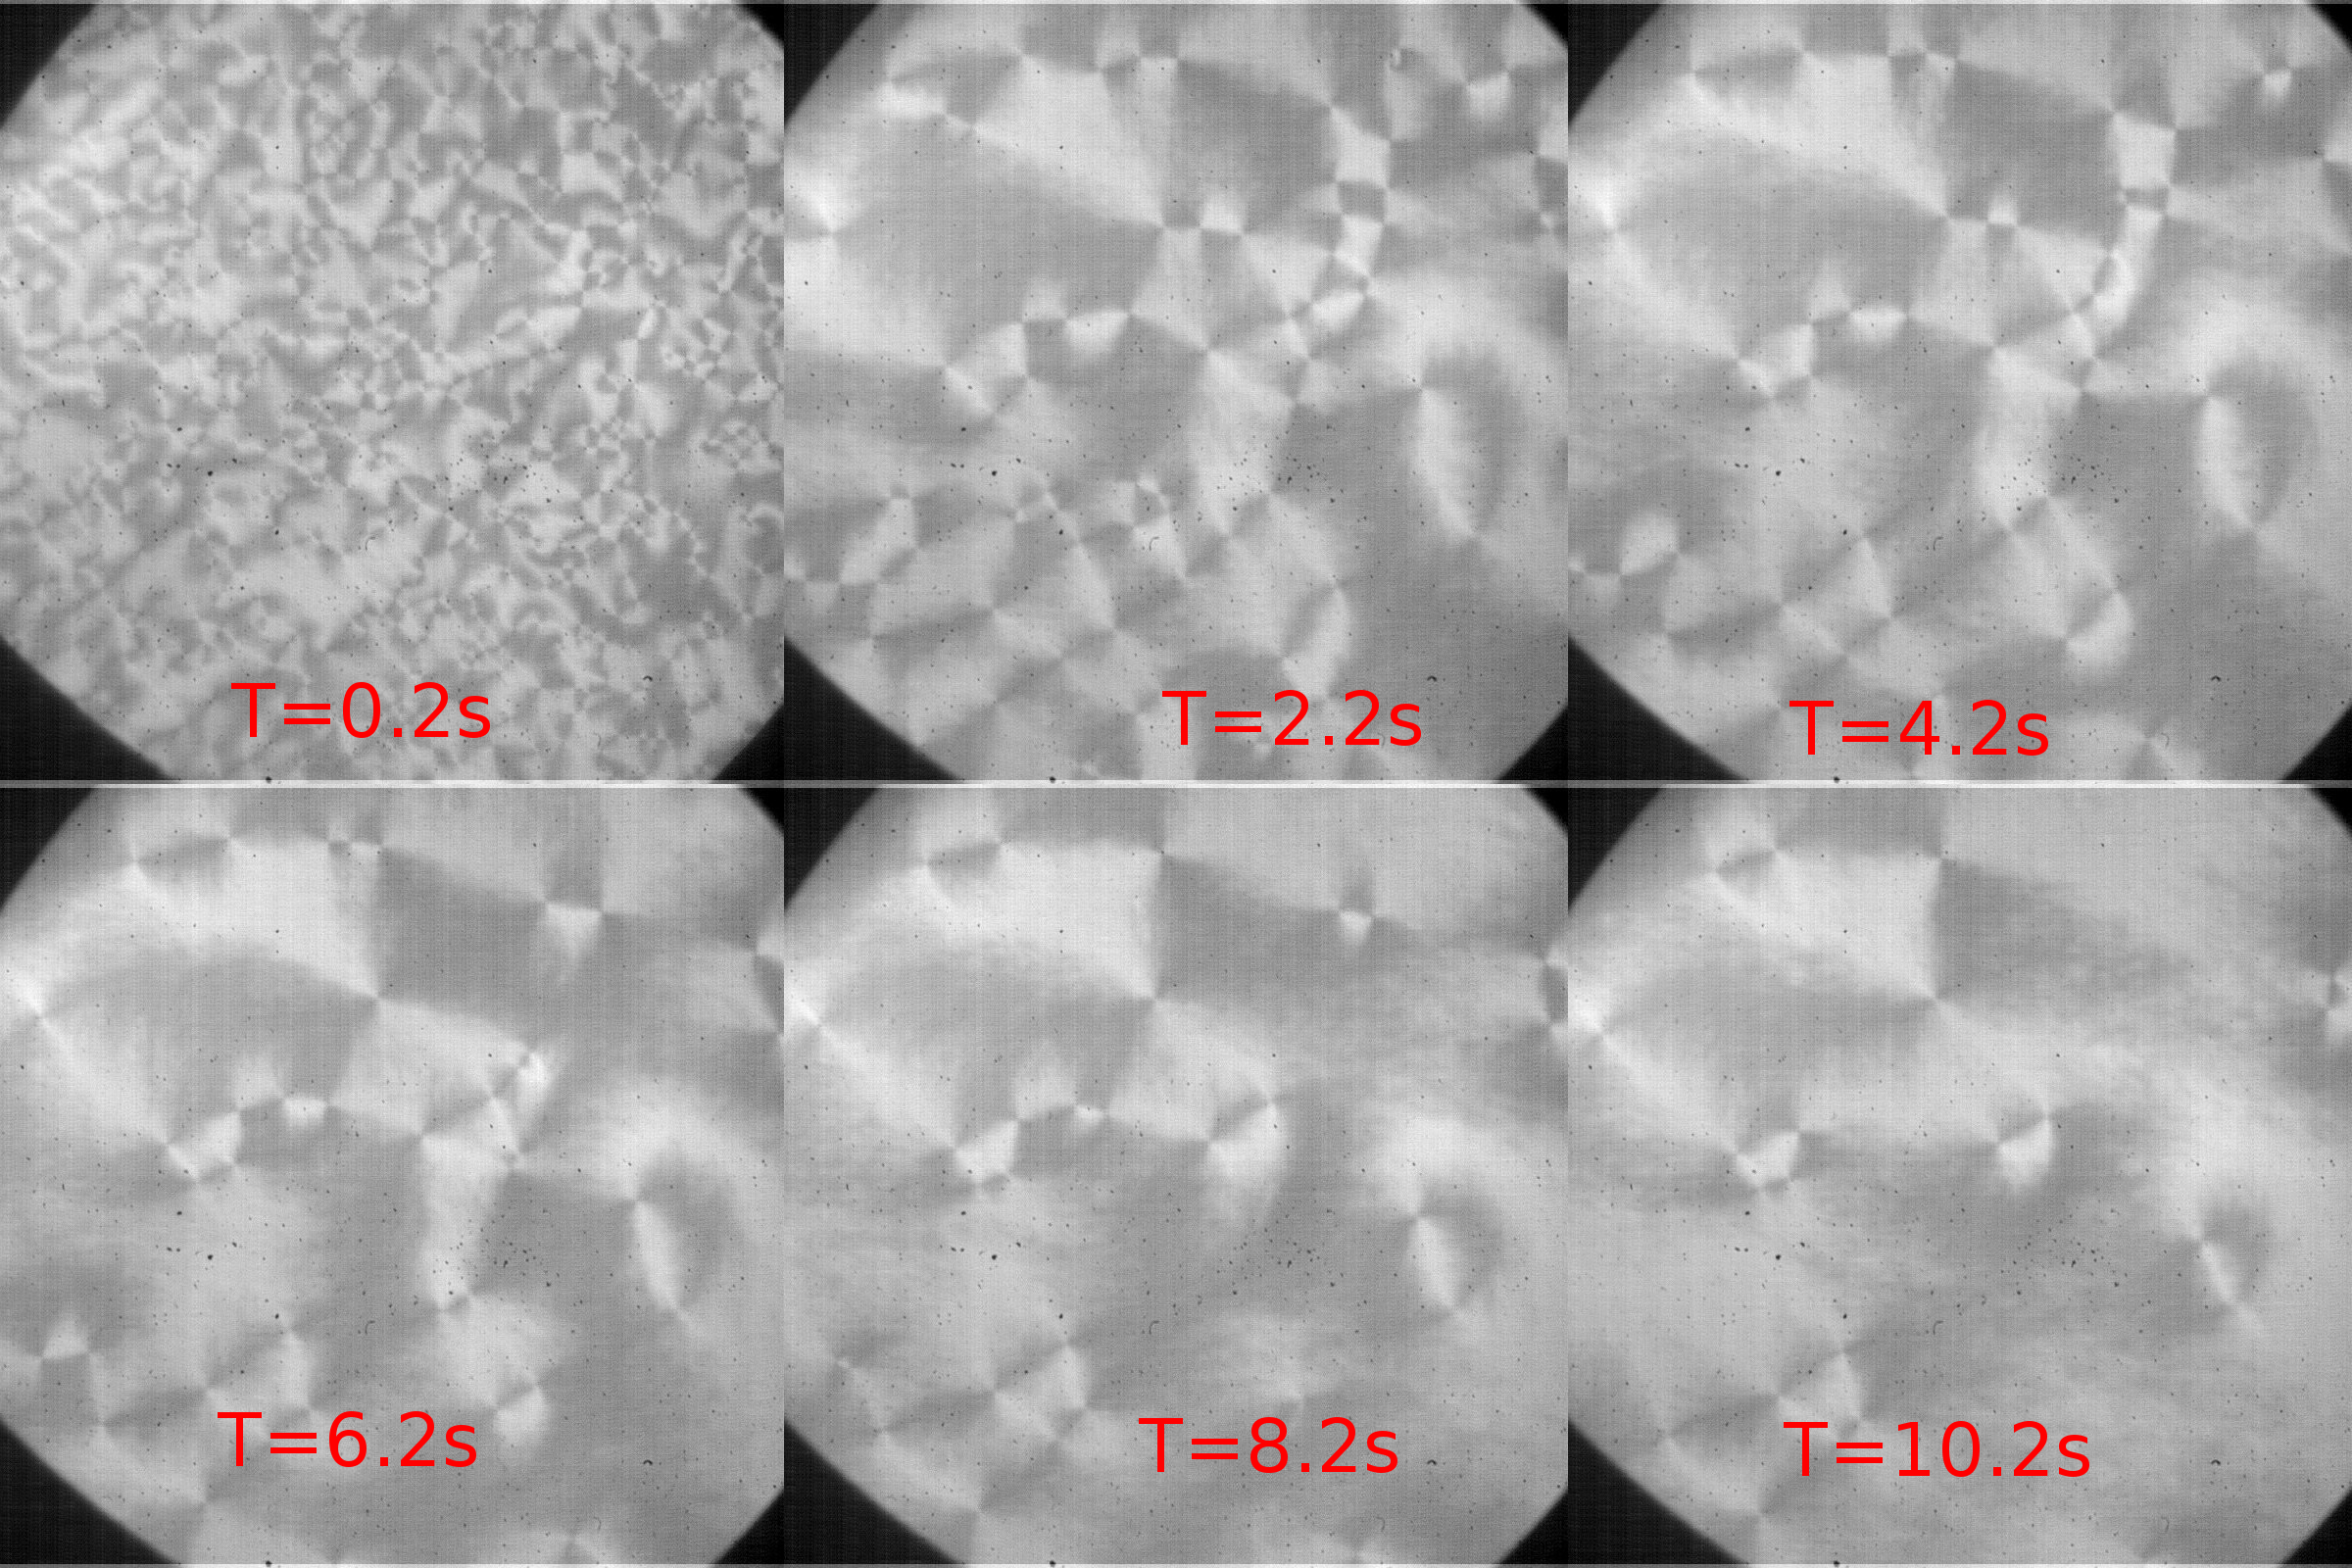
\includegraphics[width=\linewidth]{film.png}
  \caption{Time evolution of a film}
  \label{fig:frames}
\end{figure}

\section{Island Tracking}

Islands are frequently encountered while studying liquid crystal thin films, and are defined as the regions of the film where additional layers are present relative to the surrounding film. The extra layers provide additional reflection causing the regions to visually appear brighter -- particularly so in a black and white camera where they will appear as regions of the film with different intensities. Islands move in the film along with the surrounding fluid, allowing us to use them as markers which we can track to characterize the flow of the fluid film.

There are two main techniques used to identify these flows using markers: particle image velocimetry (PIV) which employs Eulerian measurement techniques, and particle tracking velocimetry (PTV) which employs Lagrangian measurement techniques. At the crux of the matter, the difference is that PIV tracks a particle through time to determine flow, while PIV identifies flow by measuring marker movements at specific locations, but not worrying about where the markers came from or goes to in the future. In previous experimentation, we have used both PIV (OpenPIV) and PTV (racetrack experiment) to identify flow in liquid crystal films, with varying results. Considering they rely on a high degree of accuracy in particle characterization in images, these tools are highly rigid and specialized placing restriction on how and what data we can analyze. 

Employing machine learning, we hope to overcome some of the limitations of these methods by simplifying the process of tracking markers in varying image qualities and conditions. A machine learning algorithm trained to identify islands of multiple sizes, intensities, shapes, and lighting conditions that would traditionally inhibit the capabilities of standard identification algorithms. 

\subsection{Simulation Data}

Considering the relative simplicity of visually identifying islands in an image, the simulation aspect for this is very straight forward. Images were prepped by generating a random number of islands with random size and intensity on a picture (We haven't actually trained anything yet, so we still need to figure out if we even need any additional noise). Several thousand of these images can be easily and quickly generated, with perfect training annotations of island locations and sizes.

\begin{figure}
  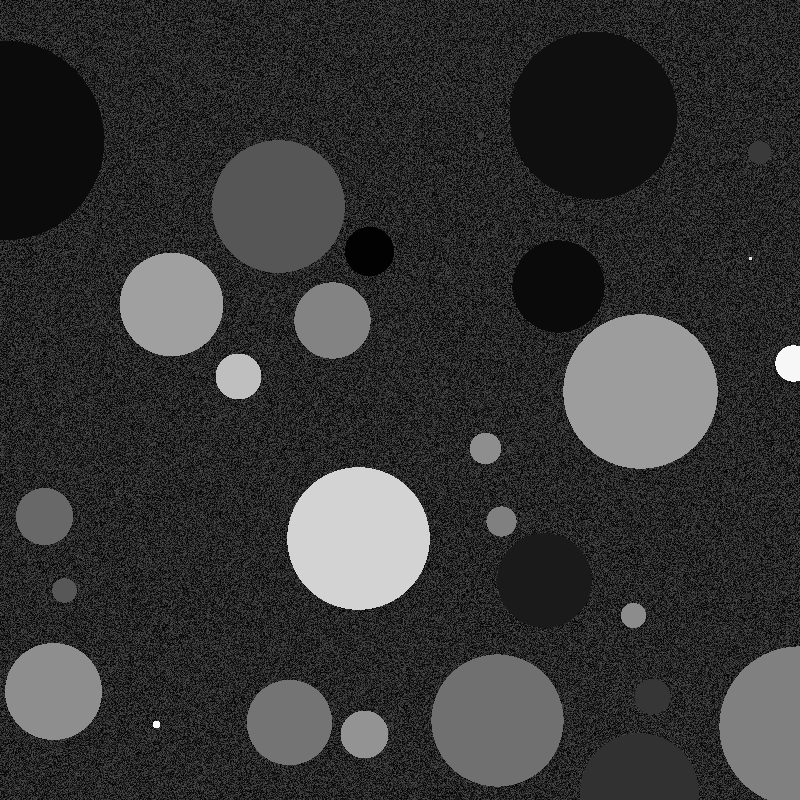
\includegraphics[width=\linewidth*3/4]{island_0024.png}
  \caption{Island training image}
  \label{fig:Islands}
\end{figure}

\section{General Object Tracking: Topological Defects}

While the island tracking with machine learning was largely successful, it is also a largely simple problem. Islands are easy simulate, simple for a human to see, and simple for a computer to identify. In order to test the system on a more complex system with complex applications, we will also try to develop the machine learning algorithm to identify the number, and location, of topological defects in images. This will require more work to make simulation images 

\subsection{Simulation Data}
%\ Need Adam to help with this section

Two methods were used to generate images for training the YOLOv2 models to detect topological defects. The first method randomizes defect count and location outputs a Schlieren texture with defects in the given locations. This method is able to output very clean, perfectly annotated images, however it only produces and image with a corresponding Schlieren texture rather than simulating the physics producing the image. This simulation method will be referred to as the random defect simulation.

%\begin{figure}
%  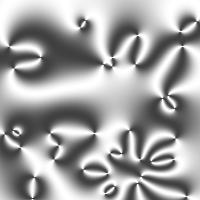
\includegraphics[width=\linewidth*3/4]{basicRD.jpg}
%  \caption{Typical image from the random defect simulation. This image used a crossed polarizer angle of 50 degrees and had the defect locations randomized.}
%  \label{fig:RandomDefect}
%\end{figure}

The second method was based on a Landau-Ginzburg implementation of the XY model. In the initial state, the C-director of each pixel is chosen randomly. The simulation is then allowed to evolve over time resulting in defects forming and annihilating naturally. This method also gives thermal noise to the system, increasing the similarity of the output images to experimental images.


\begin{figure}
  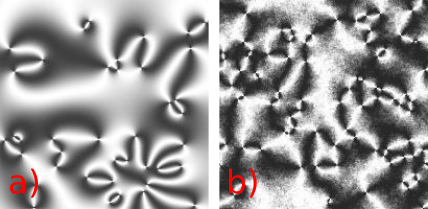
\includegraphics[width=\linewidth]{simulations.png}
  \caption{Typical image from simulation. a) uses a crossed polarizer angle of 50 degrees and randomized defect locations. b) uses an XY model where defect count decreases over time}
  \label{fig:RandomDefect}
\end{figure}
%\begin{figure}
%  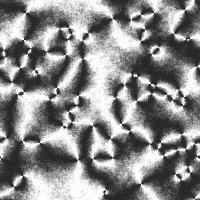
\includegraphics[width=\linewidth*3/4]{basicLG.jpg}
%  \caption{Typical image from the Landau-Ginzburg simulation. This image used a crossed polarizer angle of 50 degrees and shows thermal noise.}
%  \label{fig:Setup Sketch}
%\end{figure}

Previous work has been done demonstrating the viability of using machine learning to identify whether a given simulated photo contains a topological defect [citation]. However, the system was only run on simulated images and did not identify the locations of defects in the images, limiting its usefulness for experimental purposes. In order to make a system viable for usage with real experiments, we developed a pipeline that makes use of modern deep-learning object detection and image enhancement techniques. 

\subsection{Pipeline and Image Enhancement Motivation}

For object detection we used darkflow, which is a TensorFlow implementation of the YOLOv2 algorithm [citation]. YOLOv2 learns to perform both region-proposal and region classification using the darknet-19 architecture. Allowing the region proposal mechanism to be trained is important for our task of defect identification as object detection algorithms that rely on traditional heuristic searches, such as R-CNN [citation], would likely fail to identify the central point of a defect as an object. Training darkflow on a set of 100 simulated 200x200 images with each image containing 20 defects showed that this network is viable for detecting the locations of defects in simulation data. However, the network trained on the pure simulated data was unable to identify defects in experimental images until data enhancement techniques were used to improve the utility of the simulation images.

FIGURE

Machine learning algorithms, by nature, optimize themselves to perform as well as their architecture allows on the given training data. While this can lead to highly effective systems, it is the primary reason why training on a set of simulated data often makes the final model non-viable for usage in the real world; simulated data is highly predictable and clean while real world data can have large amounts of noise and significant variance in how certain key objects appear. By training on the simulated data, the system will over-fit on the very specific shapes, colors, and gradients produced by the simulation. Since the objects of interest in the experimental data are almost guaranteed to not be as perfect as the ones in the simulation, the machine learning model will fail to identify them. Our solution to this problem is to introduce various inaccuracies, which mimic real-world inaccuracies, into the simulated images, with the goal of making the final model more robust.

\subsection{Standardization and Simulated Image Enhancement}

The first issue that needs to be dealt with is lighting and contrast. In simulated defect images, the intensity of a pixel ranges from perfectly black to perfectly white depending on the director orientation, maximizing the gradients and contrast in the image. The mean intensity of the image will also generally be around 0.5 on a scale from 0 to 1, since there is no offset to the image brightness. When using an experimental image, the difference in brightness between perfectly aligned and perfectly misaligned directors is much smaller than the full dynamic range of the image, causing much smaller gradients. The average brightness of the experimental data is rarely 0.5, so what constitutes bright and dark pixels is more complex than just the intensity of the pixel. To make the simulation and experimental images as similar as possible in regards to average intensity and dynamic range, a common standardization procedure is used. Each pixel's intensity value is set according to the feature standardization formula 

$$ x' = \frac{x - \Bar{x}}{6\sigma} +0.5 $$

where x' is the output pixel intensity, x is the input intensity of each pixel and sigma is the standard deviation of the image pixel intensities. The output pixel intensities now have a mean of 0.5 and a dynamic range of six standard deviations. This procedure reasonably standardizes the lighting and contrast of the images regardless of the actual lighting and camera conditions.

In machine learning, training data is traditionally a hand labelled subset of the larger data-set to be analyzed. We, however, are attempting to train our algorithm with auto annotated simulation data that is more perfect than the experimental data. By adding imperfections to the simulation images, we hope to emulate the experimental data and improve the abilities of the neural network.

Due to the relatively low lighting on the images, the camera read noise, generated by the camera hardware, is significant relative to the signal size. Applying a 2-D discrete Fourier transform, the composition of the image is extracted in the frequency domain (Figure Reference). The high frequencies in the corners contain the information of interest, while the periodic read noise appears as regular lines. Removing the higher frequency spaces, the inverse Fourier transform yields the actual noise pattern of the camera. This characteristic camera noise can then be added as high-frequency noise to the simulated data set to improve veracity to real experimental data.

\begin{figure}
  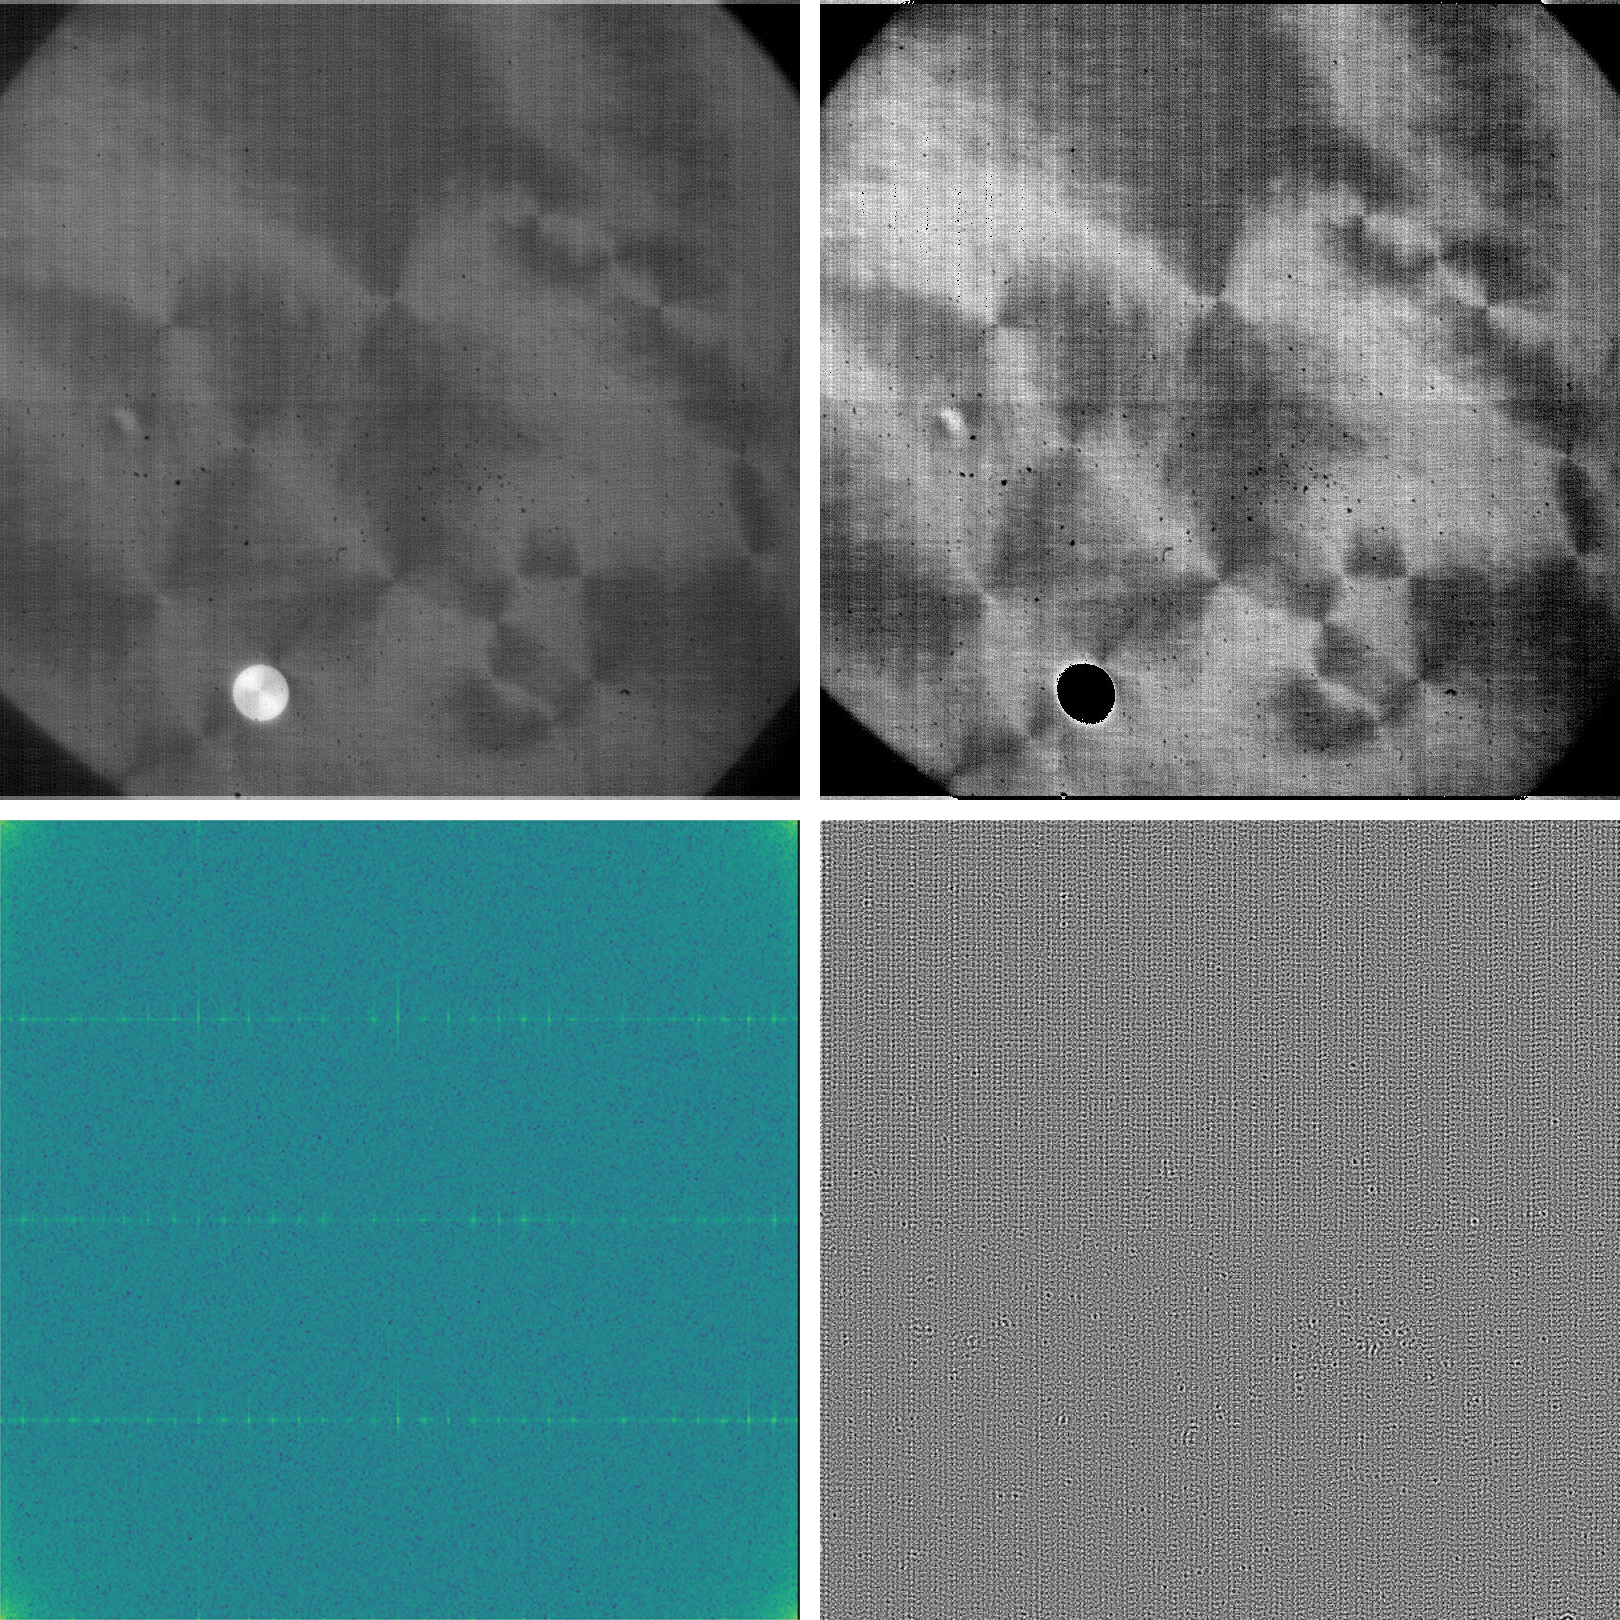
\includegraphics[width=\linewidth]{Standardizationandnoise.png}
  \caption{Image standardization and periodic noise extraction. Top-Left: Raw image. Top-Right: Standardized image. Bottom-Left: Fourier transform of standardized image. Bottom-Right: Noise extracted from the image.}
  \label{fig:Standardization and Noise}
\end{figure}

To further improve the simulation images, randomized Gaussian blurring is used to emulate the non-perfect and variable focus of the experimental data. Additionally, the overall brightness and dynamic range of the simulated images is randomized to prevent the model from being dependant on specific intensities or gradient magnitudes unique to the simulation.

The final components added to the simulated images were randomized lighting domains and circular artifacts. Observing the pattern of defect detections from previous models, it was discovered that detections would be made along lines where the lighting abruptly shifts. The microscope aperture and the boundaries between CCD sectors, which consistently read different pixel intensities, repeatedly generate such light shifts. To prevent this, the simulation images were broken into four quadrants of randomized size, with each quadrant having slightly different brightness. False detections would also be made around the boundaries of islands, which are circular objects present in liquid crystal films. To avoid this, circles of random brightness were added to the simulation data to provide negative counterexamples of non-defect objects that should be ignored.

\begin{figure}
  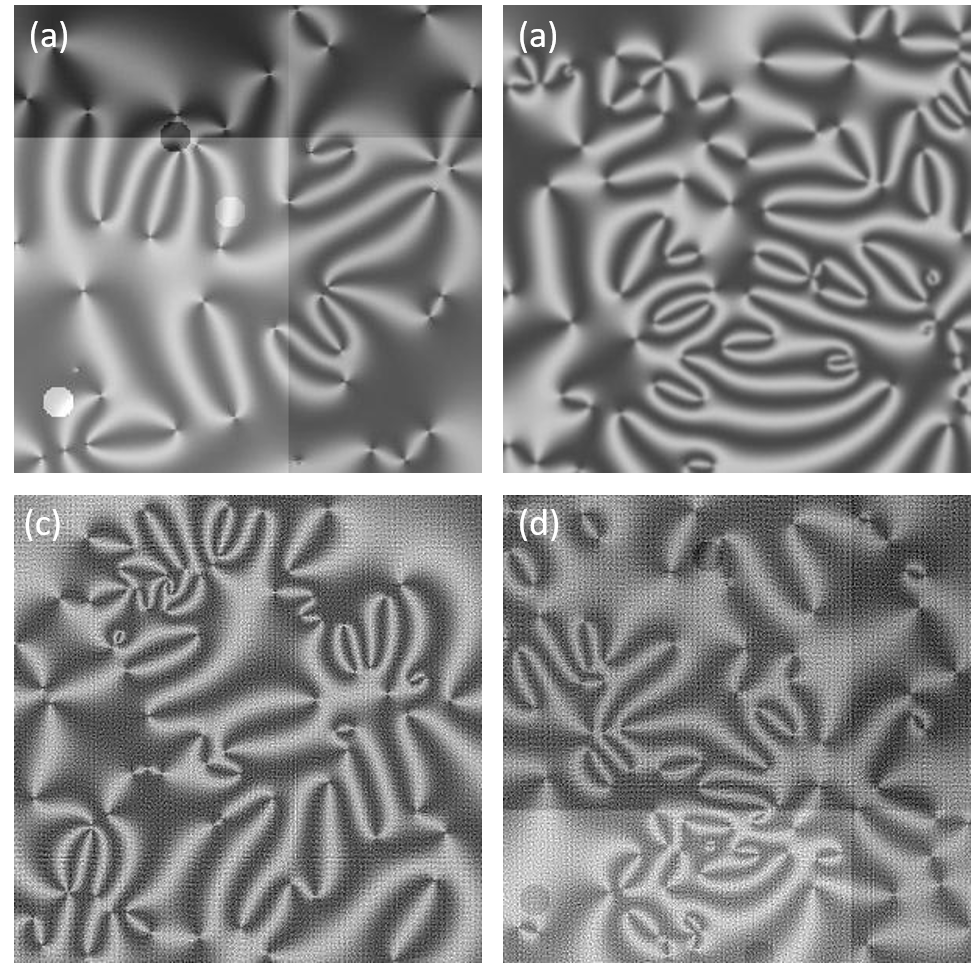
\includegraphics[width=\linewidth]{imageEnhance.png}
  \caption{Simulated images enhanced with various types of noise. (a) Image with dramatic lighting shifts and added circles (islands) (b) Image with Gaussian blurring (c) Image with Fourier noise (d) Image with all three}
  \label{fig:Standardization and Noise}
\end{figure}

\subsection{Effects of Simulated Image Enhancements}

In order to evaluate the effectiveness of each component in the pipeline, several models were trained on simulated images enhanced by the individual pipeline components. The models were validated using a hand annotated set of experimental images in order to determine how well they performed on real data relative to a human performance.

In machine learning, there are multiple metrics used to determine how well a model performs. Many of these metrics are optimized to measure the performance of specific aspects of the model ranging from accuracy, precision, recall, absolute error, etc. In our use case, we're interested in our model performing well in two aspects: accuracy, how reliable/close are our object detections, and recall, how many of the objects do we count. Both the mAP and F1 score provide a measure of these performances, relying on the Precision and Recall of a model.

\begin{figure}
  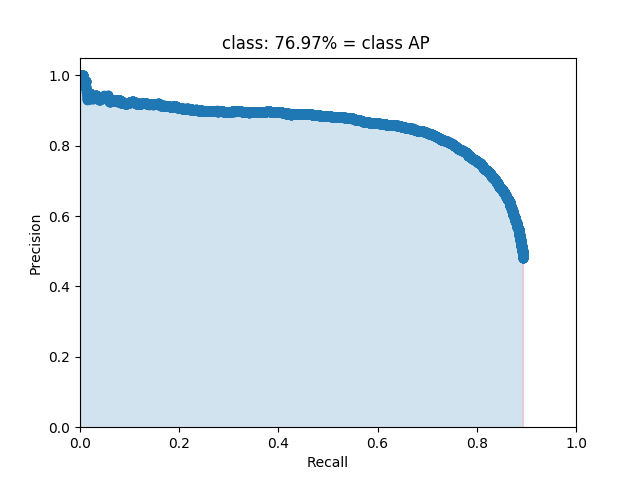
\includegraphics[width=\linewidth]{mAP.png}
  \caption{Precision-Recall plot. mAP score is the percentage of area shaded between (0,0) and (1,1)}
  \label{fig:Standardization and Noise}
\end{figure}

$$ Precision = \frac{TP}{TP+FP} $$
$$ Recall = \frac{TP}{TP+FN} $$
$$ F1 = 2*\frac{Precision * Recall}{Precision + Recall} $$
$$ AP = \int_0^1 \!p(r) \, \mathrm{d}r $$
%We need a method for explaining, simply, what the mAP score is. I dont' think the $$ AP = \int_0^1 \!p(r) \, \mathrm{d}r $$ is appropriate as it isn't exactly the mAP.... There's a difference. Perhaps with a mAP graph saying shaded area is the mAP score?

Simulated training images enhanced with blurring, random islands, random lighting quadrants, or randomized image brightness and contrast produced models that performed poorly on experimental images. On validation, these models received mAP scores of $<30\%$. Simulated images enhanced only with noise extracted using the Fourier transform produced a viable model, however the mAP score only reached $53.3\%$.

Adding multiple types of noise to the simulated images produced greatly improved models. Combining all types of artifacts produced a model with a mAP score of $61.3\%$, however this was outperformed by a model trained using only Fourier noise and randomized blurring which achieved a mAP score of $74.4\%$. Adding all forms of noise at a lower intensity to the simulated images produced a model with a mAP score of $75.4\%$.   

\begin{figure}
  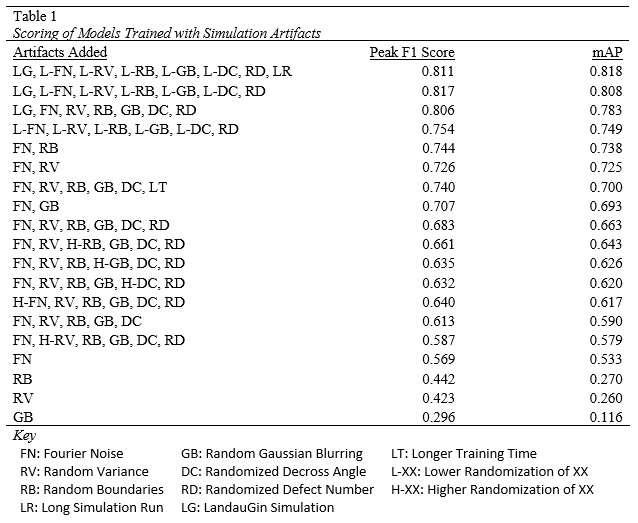
\includegraphics[width=\linewidth]{modelTable.PNG}
  \caption{mAp and peak F1 scores of models trained using simulated images trained with various combinations of artifacts.}
  \label{fig:frames}
\end{figure}

The original YOLOv2 paper reported an average mAP score of $73.4\%$ when tested using the Pascal VOC2012 test set, which puts the detection accuracy of our model trained with simulated images on par with models trained using real images. 
This supports the viability of training YOLO object detection models based on simulated data for use on experimental data.

\subsection{Improvements Using the XY Model}
Training was also performed on data from the XY model simulation, yielding improved accuracy for the final models. Without adding any artifacts, a model trained on simulated images from the XY simulation attained a $51.1\%$ mAP score, which is much higher than the model trained on the raw random defects data. 

% I don't know the exact specifications of ForLL, however I believe it's the reduced artifacts on the Long Time Fortran simulations

The LandauGin simulations are highly time dependent with defect count following a power function. This implies that it takes an order of magnitude of simulation time to generate images with significantly reduced defect counts. If we were to train a model with only early time simulation images, where there is a high density of defects in the training data, then the model will struggle to locate defects when they are less dense. As such, the best performing model required significant simulation times to generate training data with a wide variety of defect counts and densities. 

Similar to the earlier simulation data, the best results were attained with a lower intensity of many different forms of noise, achieving a mAP score of $77.0\%$. This model proved to be capable of both locating and counting the defects in our real experimental data over multiple videos with comparable performance to human counting. 

\begin{figure}
  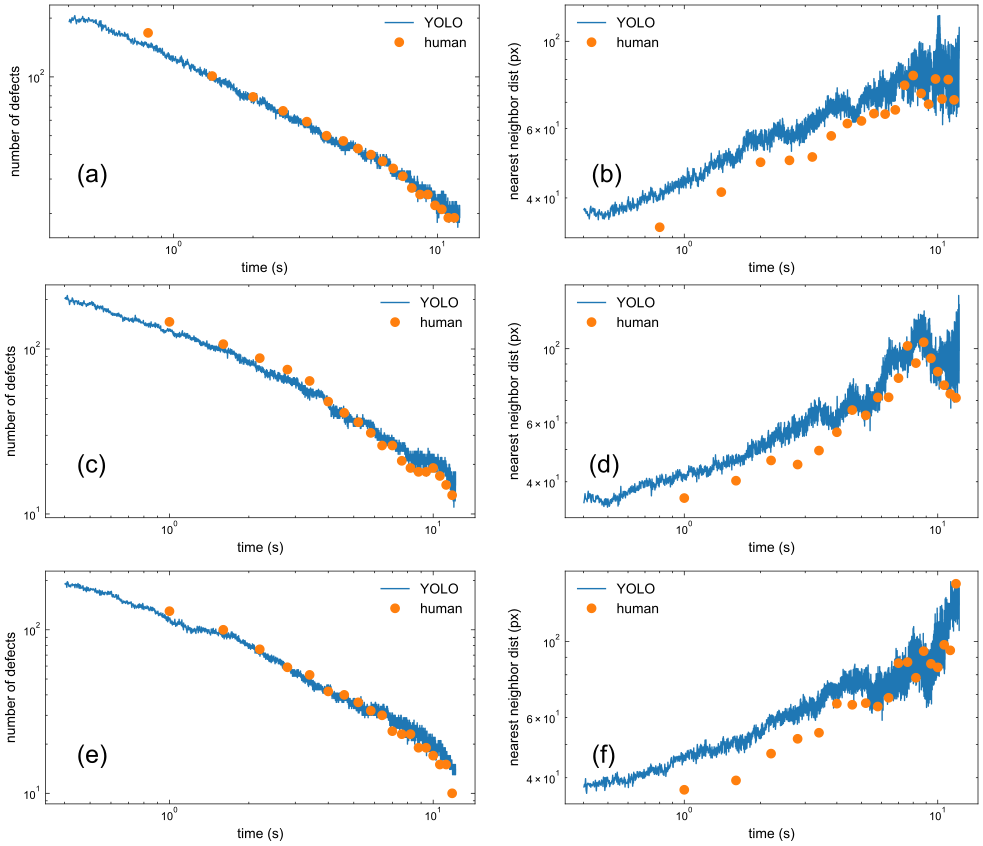
\includegraphics[width=\linewidth]{humanVmachineAllR.png}
  \caption{Number of Defects Vs. Time and Nearest Neighbour Vs. Time for 3 different videos.}
  \label{fig:HumanVMachine}
\end{figure}

The second goal, and probably the tougher goal, of the model is defect tracking. Reliable defect tracking requires that the model is consistently capable of precisely locating defects over a larger number of frames -- a challenging prospect. We made use of the Trackpy Python module, a package of functions specializing in particle tracking, to link defects through consecutive images over time. The result is a path of the defects through time.  

\section{Results and Discussion}
\blindtext{}

%\begin{figure}[H]
%\centering
%\includegraphics[keepaspectratio=true,width=\columnwidth]{fig1-jem.png}
%\caption{write figure caption here}
%\label{fig:labelfighere}
%\end{figure}
%
%\bibliographystyle{apsrev4-1}
%\bibliography{../bibfilenamewithout.bib} % this is .bib file

\end{document}